\documentclass[11pt]{article}

\usepackage[a4paper, margin=2.3cm]{geometry}
\usepackage{graphicx}
\usepackage{setspace}
\usepackage{amsmath}
\usepackage{parskip}
\usepackage{float}
\usepackage{booktabs}
\usepackage{caption}
\usepackage{microtype}
\usepackage{url}

\onehalfspacing
\graphicspath{{figures_fp/}{../figures/}}

\begin{document}

\noindent
\begin{tabular}{ll}
\textbf{Student Names:} & Mariia Solodiankina, Shengli Zhu \\
\textbf{Course:} & Geo-Environmental Modeling and Analysis \\
\textbf{Instructor:} & Prof. Hylke Beck, Prof. Yoshihide Wada \\
\end{tabular}

\vspace{0.6cm}

\begin{center}
{\Large \textbf{Climate Controls on Runoff Across Hydroclimatic Regimes Using ERA5-Land and Machine Learning Analysis}}

\vspace{0.2cm}
\textit{Final Project Report}  
\end{center}

\vspace{0.4cm}

% =======================================================================
\section{Introduction}

\subsection{Problem definition and literature review}

Whether climate change strengthens or weakens runoff depends on whether a catchment is water- or energy-limited, yet the relative importance of individual climate drivers along this continuum is rarely quantified within a single, internally consistent dataset. Classical hydroclimatology organises catchments along an aridity gradient~\cite{budyko1974}: water-limited systems lose most precipitation to evapotranspiration, while energy-limited systems receive precipitation in excess of atmospheric demand and generate sustained runoff. The Budyko framework captures, in two non-dimensional ratios, how the partitioning of precipitation depends on the balance between water supply and atmospheric demand. What it does not specify is which underlying climate variables drive catchment-scale runoff variability, nor how their relative weight shifts across regimes.

Most existing rainfall--runoff studies have addressed this gap one regime at a time -- for individual basins, for a single climate zone, or for a fixed product such as a national gauge network -- and trends in precipitation, evapotranspiration, and discharge are typically reported separately. Comparisons that hold both the dataset and the methodology fixed across fundamentally different regimes are still relatively uncommon, partly because long, internally consistent datasets covering radically different climates have only recently become available, and partly because per-sample attribution requires methods that go beyond linear regression and global feature-importance scores.

Earlier work has extended the Budyko framework with additional catchment- and climate-specific parameters~\cite{roderick2011}, and has separated climate from direct human impacts on streamflow within a single national network~\cite{wang2011}. Machine-learning approaches have entered hydrology more recently and frequently outperform traditional rainfall--runoff models for streamflow prediction, but their black-box nature has limited their use as scientific tools~\cite{nearing2021}. Tree-exact SHAP partly addresses the interpretability gap by decomposing each individual prediction into per-feature contributions; in this comparative form -- across regimes spanning the global aridity continuum -- we have seen relatively few applications to runoff attribution.

Two recent developments narrow this gap. The ERA5-Land reanalysis~\cite{munoz2021era5land} provides a 76-year, physically consistent record of precipitation, evapotranspiration, runoff, soil moisture and energy-balance variables at 0.1$^\circ$ resolution, allowing the same closed water balance to be evaluated in the Sahara, the Po Valley and the Ganges delta. Gradient-boosted trees~\cite{xgboost2016} combined with Shapley-value attribution~\cite{lundberg2017shap,lundberg2020shaptrees} now allow each climate variable's contribution to an individual runoff prediction to be decomposed exactly and per-sample, rather than as a single dataset-wide importance score. Their combined use to compare runoff generation across contrasting hydroclimatic regimes, however, has so far been less common in the literature we surveyed.

\subsection{Objective and research questions}

This study quantifies how individual climate drivers control runoff across three countries that span the global aridity gradient -- Saudi Arabia (hyper-arid), Italy (semi-arid to sub-humid transitional), and Bangladesh (tropical monsoon humid) -- using ERA5-Land data for 1950--2025 and an explainable machine-learning framework. We address:

\begin{enumerate}
    \item How do water balance components and their long-term trends differ across the three regimes?
    \item Does the predictive skill of climate-to-runoff machine-learning models vary systematically along the aridity gradient?
    \item Which climate variables dominate runoff generation in each regime, and does this dominance shift with temporal scale of analysis?
\end{enumerate}

\subsection{Novelty}

This report applies SHAP attribution to the full 76-year ERA5-Land record at pixel-year resolution -- longer and more spatially resolved than the time windows used in most comparable machine-learning hydrology studies -- and reads the resulting attribution patterns through the water- to energy-limited framework, tracing how precipitation's importance shifts across the three regimes.

% =======================================================================
\section{Study Area}

The three study countries occupy contrasting positions along the global aridity spectrum (Fig.~\ref{fig:studyarea}, Table~\ref{tab:waterbalance}). Saudi Arabia is hyper-arid (K\"oppen BWh/BWk), with topography ranging from the Hijaz mountains along the Red Sea coast to the Rub'~al~Khali sand seas in the interior. Italy spans a Mediterranean (Csa) south and an Alpine--temperate (Cfa/Cfb) north, producing a marked north--south precipitation gradient. Bangladesh lies in the tropical monsoon belt (Am), dominated by the Ganges--Brahmaputra--Meghna lowlands. The three together span the water-limited, transitional, and energy-limited regimes.

\begin{figure}[H]
    \centering
    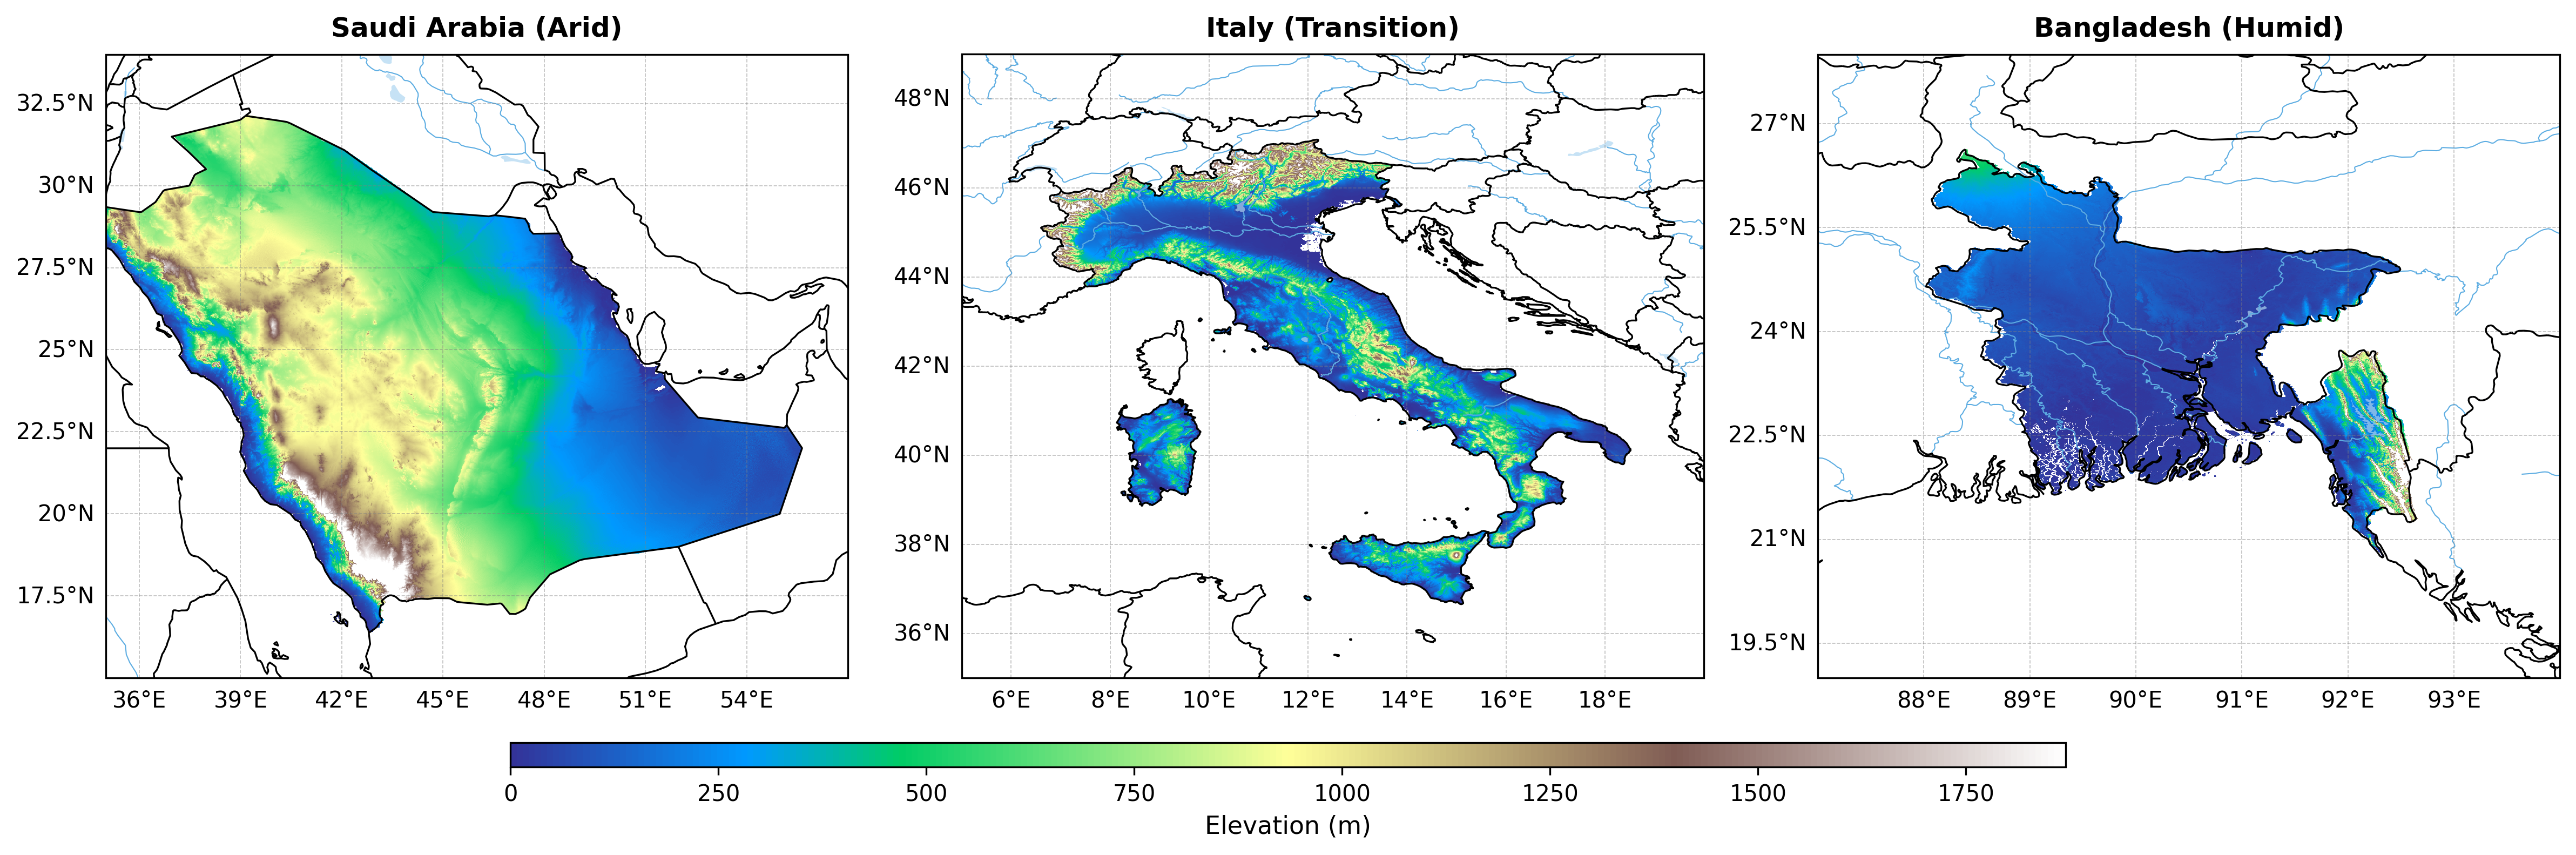
\includegraphics[width=\linewidth]{fig01_study_area.png}
    \caption{Topography of the three study regions from MERIT DEM~\cite{yamazaki2017merit}: Saudi Arabia (arid), Italy (transitional), and Bangladesh (humid). Elevation in metres above sea level.}
    \label{fig:studyarea}
\end{figure}

% =======================================================================
\section{Data and Methodology}

\subsection{Data}

All climate and hydrological variables were extracted from ERA5-Land Monthly Aggregated (\texttt{ECMWF/\allowbreak ERA5\_\allowbreak LAND/\allowbreak MONTHLY\_\allowbreak AGGR}) via Google Earth Engine, covering February 1950 to December 2025 (911 months) at 0.1$^\circ$ native resolution. Precipitation, evapotranspiration, surface and subsurface runoff, and four layers of volumetric soil water content were used to close the water balance. Air temperature, dewpoint temperature, net short- and long-wave radiation, 10~m wind speed, soil temperature, and soil water storage change provided the predictor set for the attribution analysis. Terrain data for study-area visualisation were obtained from the MERIT DEM v1.0.3~\cite{yamazaki2017merit} at 3~arc-second resolution. Country boundaries were taken from FAO GAUL 2015 and used to clip each variable to the national polygon.

\subsection{Water balance}

The monthly water balance at the national mean scale was evaluated as
\begin{equation}
P = ET + R + \Delta S + \varepsilon,
\end{equation}
where $P$, $ET$, $R$ denote monthly precipitation, actual evapotranspiration, and total runoff (surface plus subsurface), and $\Delta S = S(t) - S(t-1)$ is the change in total soil water storage computed from the depth-weighted sum of four ERA5-Land layers ($S_1$--$S_4$, with layer weights 70, 210, 720, and 1890~mm~m$^{-3}$~m$^{-3}$). The residual $\varepsilon$ quantifies closure error. Annual aggregates were formed by summing flux variables and averaging state variables; the annual runoff coefficient is $RC = R_\mathrm{annual}/P_\mathrm{annual}$.

\subsection{Trend analysis}

Long-term trends were evaluated at both the national and pixel scales. At the national scale, non-parametric Mann--Kendall tests~\cite{mann1945} detected monotonic changes in annual and seasonal (DJF/\allowbreak MAM/\allowbreak JJA/\allowbreak SON) time series, with slope magnitudes estimated by the Sen's slope estimator~\cite{sen1968}. At the pixel scale, the same pair of tests was applied independently to each grid cell using the 76-year annual time series; pixels with $p < 0.05$ were rendered at full opacity to highlight significant spatial patterns.

\subsection{XGBoost--SHAP attribution}

Gradient-boosted regression trees~\cite{xgboost2016} were trained to predict annual runoff from eight climate features ($P$, $T$, $T_d$, net short-wave and long-wave radiation, wind speed, soil temperature, and $\Delta S$). Monthly ERA5-Land data were aggregated to pixel-year records, with flux variables summed and state variables averaged. A strictly temporal three-way split prevented data leakage: 1950--1996 for training, 1997--2004 for validation, and 2005--2025 for held-out testing. Trees were grown to depth~5 with learning rate 0.1, row and column subsampling 0.8, and a maximum of 500 rounds; training was terminated when the Kling--Gupta efficiency~\cite{gupta2009kge} on the validation set stopped improving for 20 consecutive rounds. Model performance was reported using $R^2$, RMSE, NSE~\cite{nash1970nse}, and KGE.

Feature attributions were computed with the tree-exact SHAP algorithm~\cite{lundberg2020shaptrees}. For each sample the prediction decomposes as
\begin{equation}
\hat{y} = \phi_0 + \sum_{i=1}^{n} \phi_i,
\end{equation}
with $\phi_0$ the model base value and $\phi_i$ the marginal contribution of feature~$i$. SHAP values were computed on the full annual test set, and the mean absolute SHAP value per feature was used as the cross-regime importance metric.

% =======================================================================
\section{Results}

\subsection{Water balance structure}

The three regions occupy markedly different positions on the Budyko space (Table~\ref{tab:waterbalance}, Fig.~\ref{fig:spatial}). Saudi Arabia receives only 67~mm~yr$^{-1}$ of precipitation, almost all attributed to evapotranspiration, giving a runoff coefficient of 3\%. Italy partitions intermediate fluxes ($P \approx 1{,}047$~mm~yr$^{-1}$, $RC = 41\%$). Bangladesh is strongly energy-limited, with $P \approx 2{,}316$~mm~yr$^{-1}$ and 56\% of precipitation converted to runoff. The spatial maps (Fig.~\ref{fig:spatial}) show that within-country heterogeneity is large: Saudi precipitation and runoff cluster along the Hijaz escarpment, Italian runoff concentrates in the Alpine headwaters, and Bangladesh's runoff maxima follow the Meghna flood zone in the north-east.

\begin{table}[H]
    \centering
    \small
    \caption{Multi-year mean water balance components and ratios, 1950--2025, ERA5-Land national means.}
    \label{tab:waterbalance}
    \begin{tabular}{lrrrrrr}
        \toprule
        Country & $P$ & $ET$ & $R$ & $RC$ & $ET/P$ & $R/P$ \\
                & (mm~yr$^{-1}$) & (mm~yr$^{-1}$) & (mm~yr$^{-1}$) & & & \\
        \midrule
        Saudi Arabia (arid)        & 67.1    & 72.2    & 2.5     & 0.03 & 1.11 & 0.03 \\
        Italy (transitional)       & 1{,}046.7  & 633.4   & 435.0   & 0.41 & 0.61 & 0.41 \\
        Bangladesh (humid)         & 2{,}316.0  & 1{,}052.0  & 1{,}316.9  & 0.56 & 0.46 & 0.56 \\
        \bottomrule
    \end{tabular}
\end{table}

\begin{figure}[H]
    \centering
    
\includegraphics[width=0.85\linewidth]{fig02_spatial_distribution.png}
    \caption{Multi-year mean spatial distribution of precipitation (top), evapotranspiration (middle), and runoff (bottom) for Saudi Arabia, Italy, and Bangladesh (1950--2025, mm~month$^{-1}$). Rows share a common variable; columns share a country.}
    \label{fig:spatial}
\end{figure}

\subsection{Long-term trends}

All three countries warm significantly over 1950--2025 (Table~\ref{tab:trends}). Precipitation and runoff trends are regionally specific. Bangladesh shows simultaneous declines in $P$ ($-4.15$~mm~yr$^{-1}$) and $R$ ($-3.70$~mm~yr$^{-1}$), a fingerprint of weakening summer monsoon. Italy shows a significant rise in evapotranspiration ($+0.88$~mm~yr$^{-1}$) without a matching change in $P$ or $R$. Saudi Arabia shows a weak but significant runoff decrease despite no change in precipitation.

Pixel-level maps (Fig.~\ref{fig:spatialtrends}) expose patterns hidden by national means. Italy displays a clear north--south contrast: $P$ and $R$ increase in the Alpine north and decrease in the Mediterranean south. Bangladesh's $P$ decline concentrates in the north-eastern Sylhet region, while the south-western delta shows muted trends. Saudi Arabia's significant pixels are confined to the Hijaz--Asir highlands; the rest of the peninsula has no detectable 76-year trend in $P$ or $R$.

\begin{table}[H]
    \centering
    \small
    \caption{Mann--Kendall trend test results for annual time series, 1950--2025. Sen's slope in mm~yr$^{-1}$ for fluxes and $^\circ$C~yr$^{-1}$ for temperature. Significance at $\alpha = 0.05$ (**) and $\alpha = 0.01$ (***).}
    \label{tab:trends}
    \begin{tabular}{llrrl}
        \toprule
        Country & Variable & Sen's slope & $p$-value & Sig. \\
        \midrule
        Saudi Arabia & $P$ & $-0.17$ & 0.12 & --- \\
                     & $ET$ & $-0.08$ & 0.39 & --- \\
                     & $R$ & $-0.01$ & $<0.01$ & *** \\
                     & $T$ & $+0.03$ & $<0.01$ & *** \\
        \midrule
        Italy        & $P$ & $-0.14$ & 0.85 & --- \\
                     & $ET$ & $+0.88$ & $<0.01$ & *** \\
                     & $R$ & $-0.65$ & 0.18 & --- \\
                     & $T$ & $+0.03$ & $<0.01$ & *** \\
        \midrule
        Bangladesh   & $P$ & $-4.15$ & 0.02 & ** \\
                     & $ET$ & $-0.20$ & 0.27 & --- \\
                     & $R$ & $-3.70$ & 0.02 & ** \\
                     & $T$ & $+0.01$ & $<0.01$ & *** \\
        \bottomrule
    \end{tabular}
\end{table}

\begin{figure}[H]
    \centering
    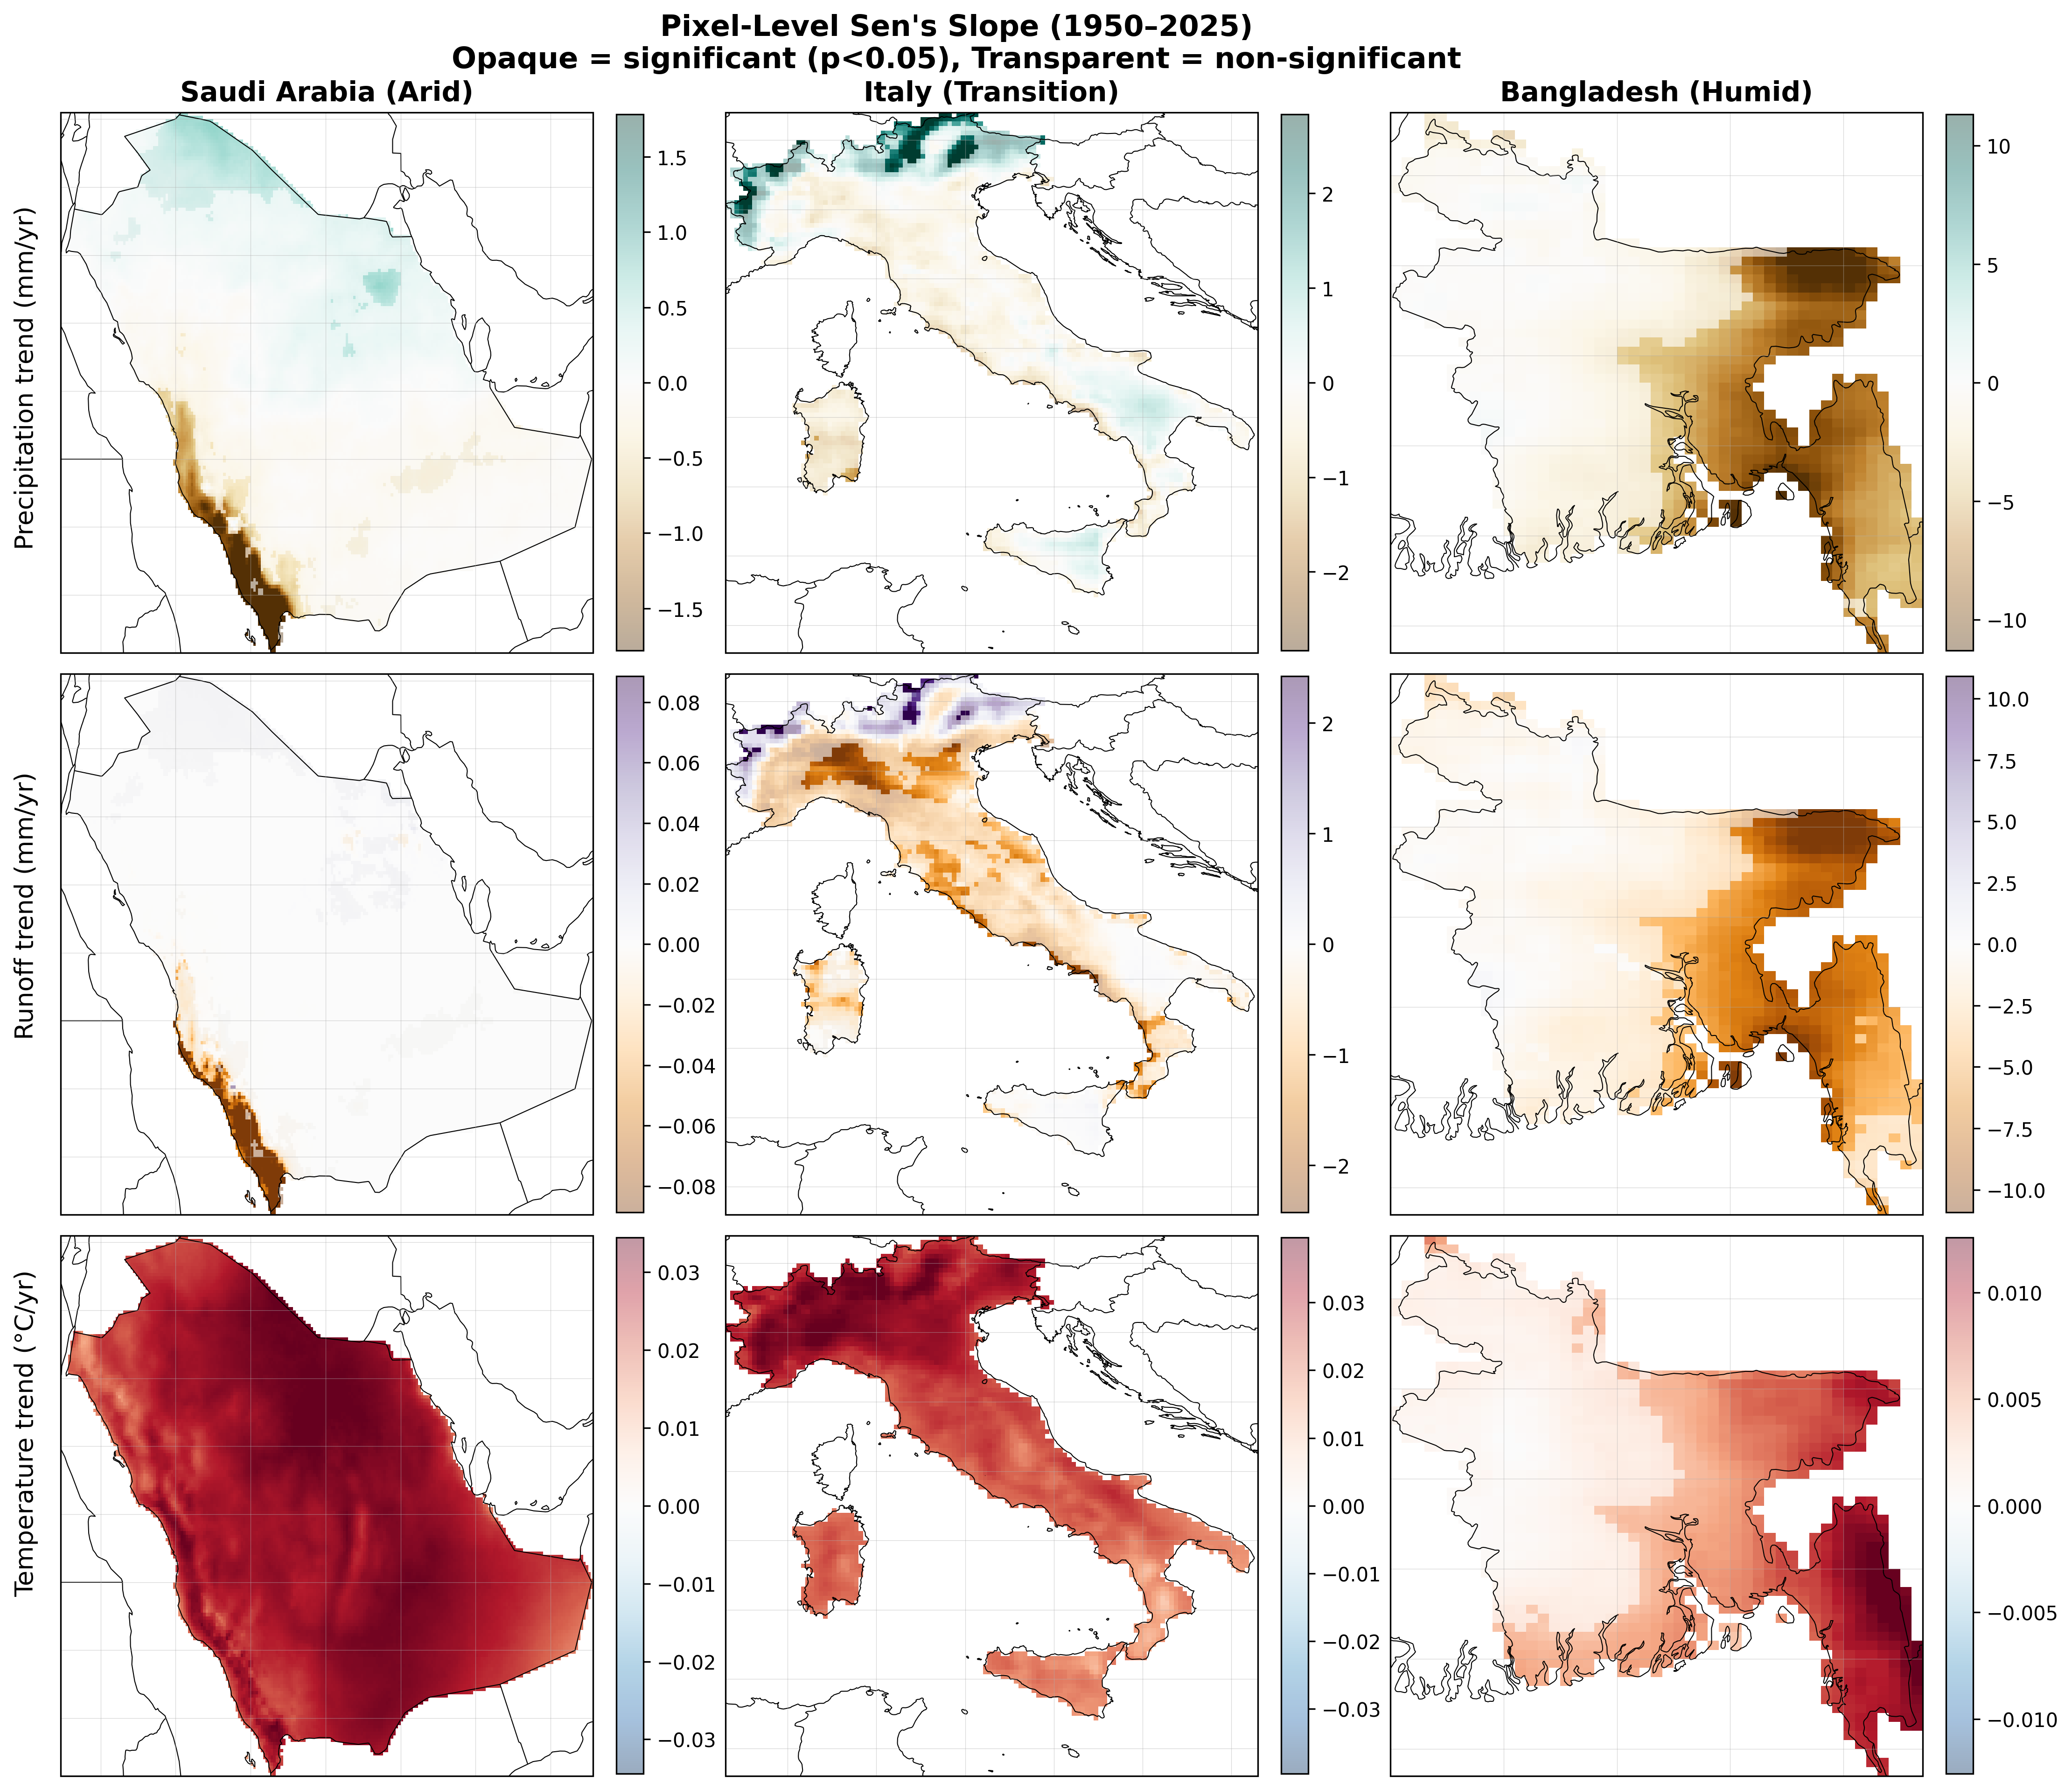
\includegraphics[width=0.9\linewidth]{fig08_spatial_trend_maps.png}
    \caption{Pixel-level Sen's slope maps for precipitation (top), runoff (middle), and temperature (bottom). Opaque pixels: $p<0.05$; semi-transparent pixels: not significant. Units: mm~yr$^{-1}$ and $^\circ$C~yr$^{-1}$.}
    \label{fig:spatialtrends}
\end{figure}

\subsection{Machine-learning skill varies systematically with aridity}

Annual XGBoost skill rises monotonically from arid to humid (Table~\ref{tab:metrics}, Fig.~\ref{fig:predobs}). Saudi Arabia reaches only $R^2 = 0.59$ ($\mathrm{KGE} = 0.69$): annual climate averages carry too little information about the rare extreme events that generate runoff in a hyper-arid environment. Italy and Bangladesh achieve near-perfect annual fits ($R^2 = 0.97$ and $0.98$), with annual runoff almost entirely predictable from annual climate variables.

\begin{table}[H]
    \centering
    \small
    \caption{Annual XGBoost predictive skill on the held-out test period (2005--2025).}
    \label{tab:metrics}
    \begin{tabular}{lcccc}
        \toprule
        Country & $R^2$ & RMSE (mm~yr$^{-1}$) & NSE & KGE \\
        \midrule
        Saudi Arabia    & 0.59 & 8.83  & 0.59 & 0.69 \\
        Italy           & 0.97 & 78.87 & 0.97 & 0.96 \\
        Bangladesh      & 0.98 & 90.07 & 0.98 & 0.98 \\
        \bottomrule
    \end{tabular}
\end{table}

\begin{figure}[H]
    \centering
    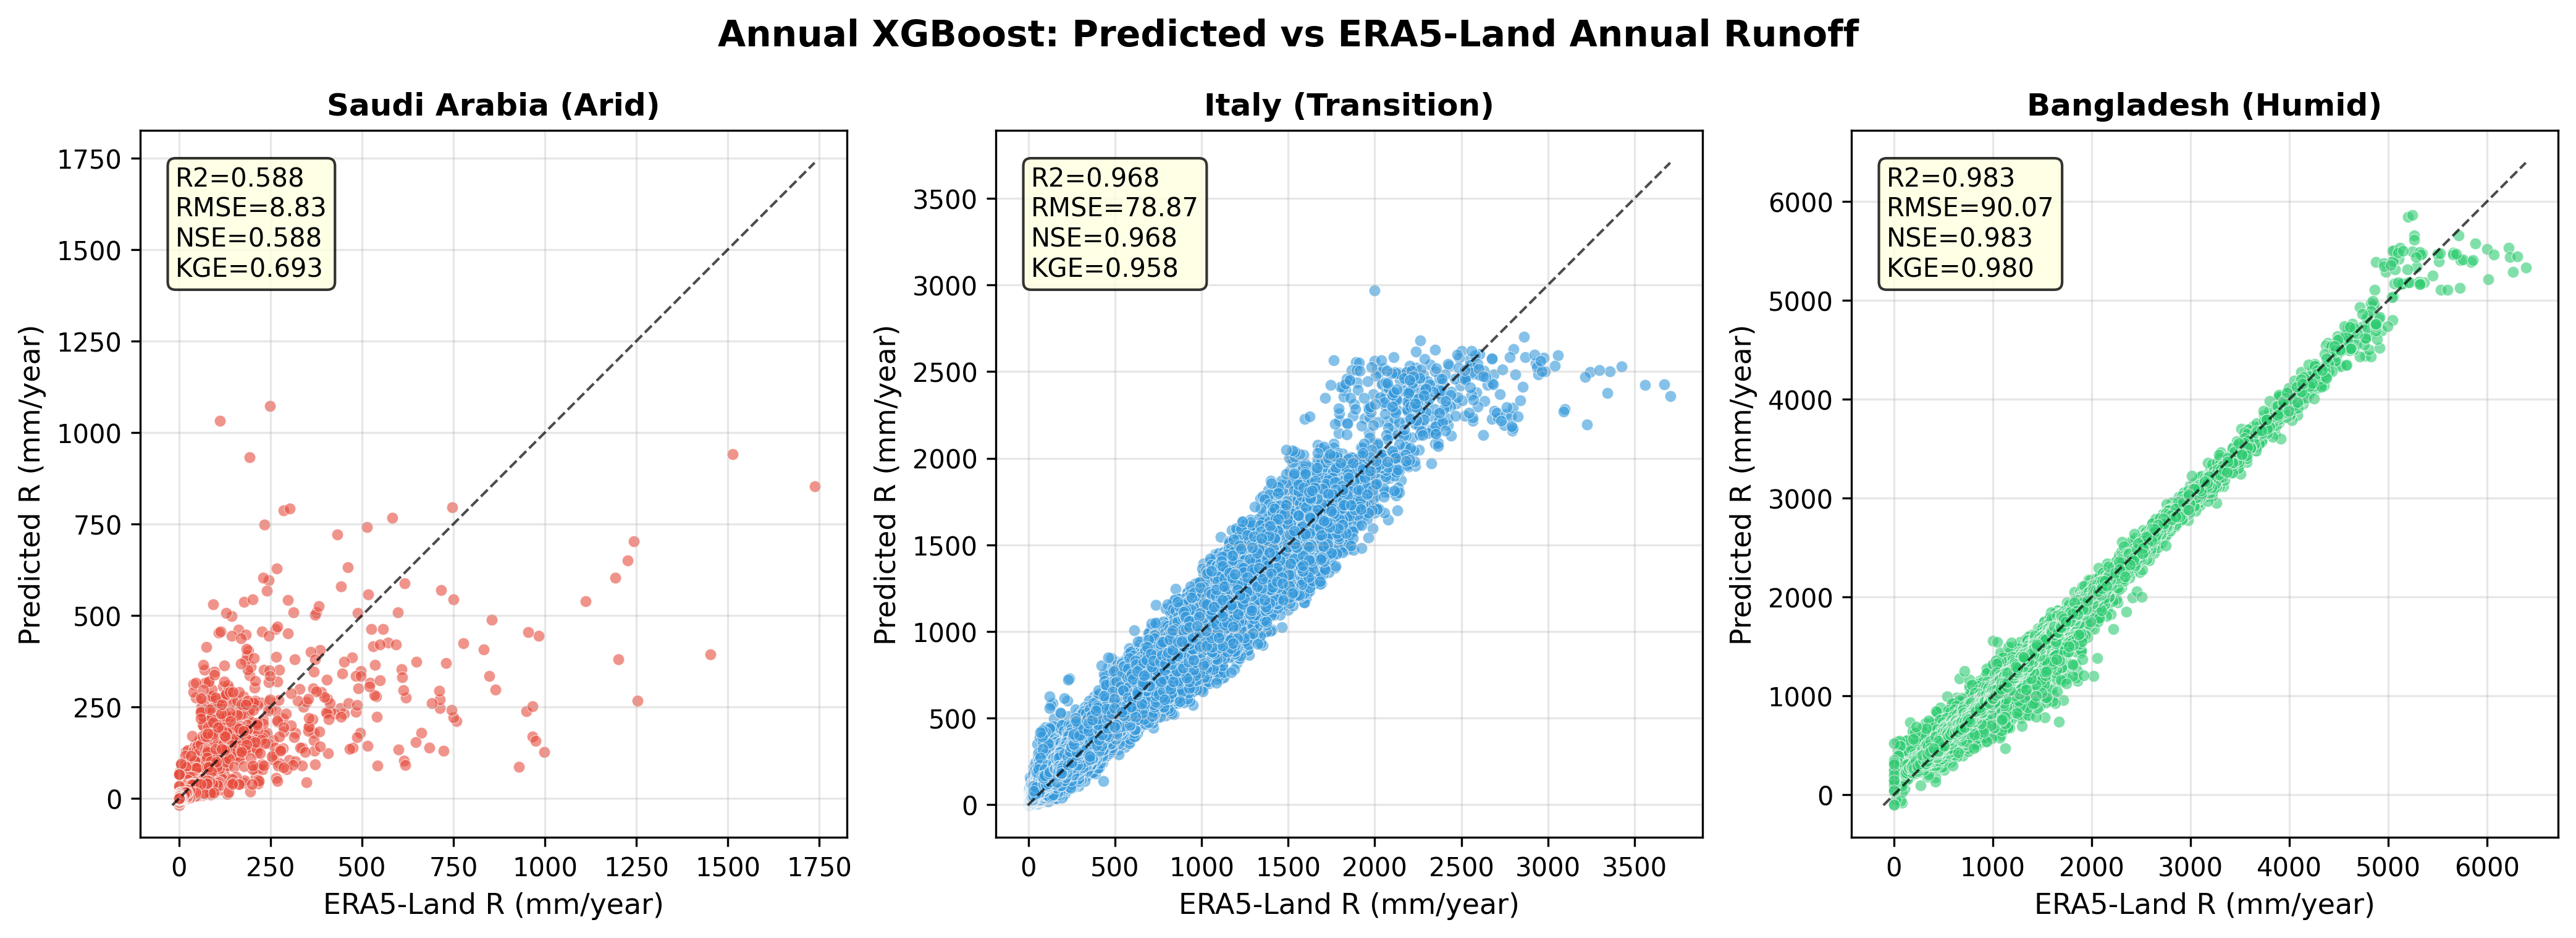
\includegraphics[width=\linewidth]{fig09b_annual_predicted_vs_observed.png}
    \caption{Annual XGBoost predictions versus ERA5-Land reanalysis runoff on the held-out test period (2005--2025). Dashed line: 1:1. Inset metrics computed on all pixel-year samples per country.}
    \label{fig:predobs}
\end{figure}

\subsection{Climate drivers of runoff across the aridity gradient}

Precipitation is the top driver of annual runoff in all three countries, but its absolute contribution spans two orders of magnitude (Fig.~\ref{fig:shapbar}). Mean $|\mathrm{SHAP}|$ for precipitation is $\sim$2~mm~yr$^{-1}$ in Saudi Arabia, $\sim$270~mm~yr$^{-1}$ in Italy, and $\sim$500~mm~yr$^{-1}$ in Bangladesh. Secondary drivers differ between regimes. In Saudi Arabia all features have small magnitude; net short-wave radiation and dewpoint temperature occupy the second and third positions. In Italy the second and third drivers are soil temperature and soil water change ($\sim$45~mm~yr$^{-1}$). In Bangladesh net short-wave radiation ranks second and soil water change third ($\sim$30~mm~yr$^{-1}$). The presence of soil water change among the top three in both Italy and Bangladesh suggests that antecedent soil conditions modulate how rainfall converts to runoff in both transitional and humid regimes, even if the mechanism is not strictly diagnostic of saturation-excess flow.

The dependence plot for precipitation (Fig.~\ref{fig:shapdep}) shows a near-linear relationship in Bangladesh, where each additional millimetre of annual rainfall adds about one millimetre of predicted runoff. Italy shows a smooth, monotonic curve: SHAP changes sign near $\sim$1,000~mm~yr$^{-1}$ -- close to the country's mean annual precipitation -- with drier pixels pulling the prediction below the model average and wetter pixels pushing it above. Saudi Arabia shows the same hockey-stick shape at much smaller magnitudes, in line with the low model skill there.

\begin{figure}[H]
    \centering
    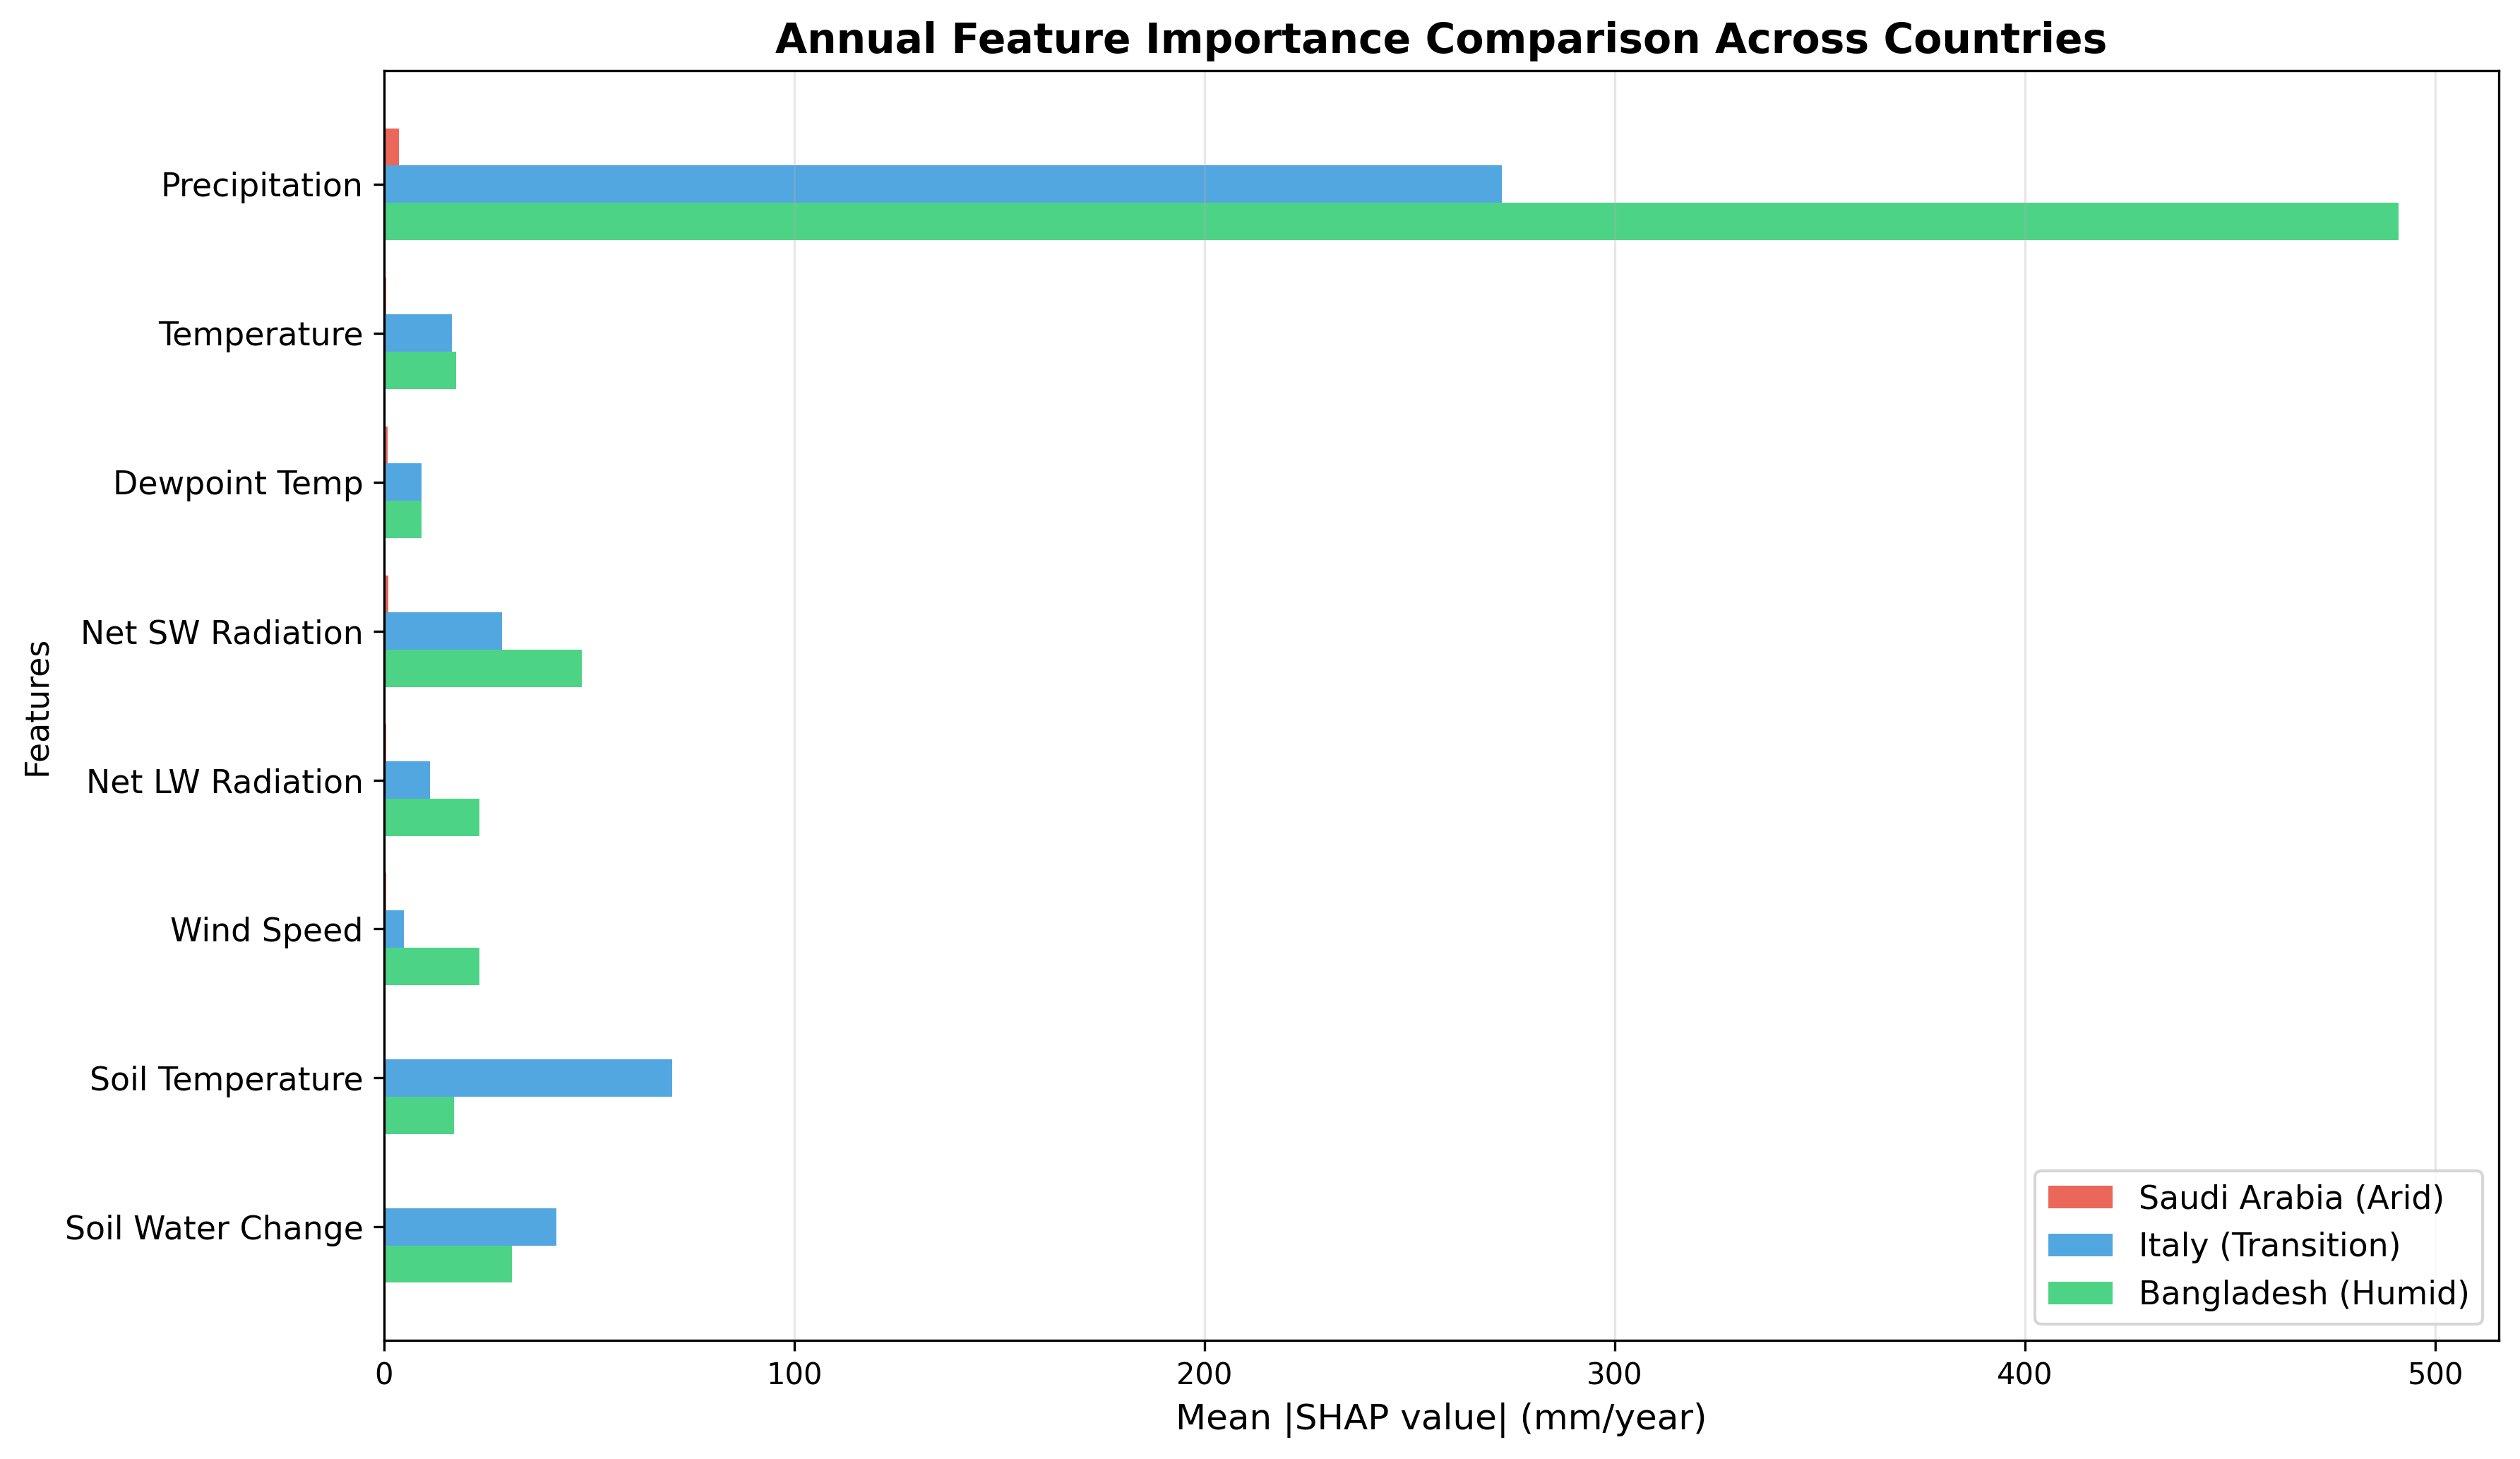
\includegraphics[width=\linewidth]{fig12b_annual_shap_bar.png}
    \caption{Mean absolute SHAP values for each climate feature in the annual model, for the three countries. Larger bars indicate stronger control on predicted annual runoff.}
    \label{fig:shapbar}
\end{figure}

\begin{figure}[H]
    \centering
    
\includegraphics[width=\linewidth]{fig13b_annual_shap_dependence_P.png}
    \caption{SHAP dependence of annual precipitation on predicted annual runoff, coloured by annual temperature. Each point is one pixel-year from the held-out test period.}
    \label{fig:shapdep}
\end{figure}

% =======================================================================
\section{Discussion}
\label{sec:discussion}

\subsection{Mechanism behind the cross-regime gradient}

The gradient has a straightforward physical interpretation. In water-limited catchments most precipitation is consumed by evapotranspiration and only rare extremes leave a runoff signal, so a single annual rainfall value carries little predictive information and any individual climate driver contributes little on average. As a system moves toward saturation, each additional millimetre of rainfall is increasingly likely to leave the catchment as runoff, the climate--runoff relationship flattens toward unity, and precipitation alone explains nearly all the variance. The transition is not a step at any particular aridity threshold but a smooth re-weighting of which variables matter and how strongly -- and the shape of the precipitation dependence plot in each country, from a hockey-stick at very small magnitudes (Saudi Arabia) to a smooth S-curve (Italy) to an almost linear response (Bangladesh), traces this re-weighting feature by feature.

\subsection{Limitations}

ERA5-Land overestimates bare-soil evaporation in hyper-arid regions; the resulting $ET/P > 1$ in Saudi Arabia is a known reanalysis artefact, and the Saudi numbers should be read as descriptive of the product rather than of the physical landscape. Fitting a single XGBoost model per country implicitly assumes that the climate--runoff relationship is spatially stationary within each polygon. This is a rough approximation for Italy, where Alpine and Mediterranean subdomains are driven by different processes, and could be relaxed by clustering pixels before model fitting. Aggregating to monthly and annual scales also removes information on sub-monthly storms, which dominate runoff in arid environments. Finally, all conclusions rest on a single reanalysis product without ground-based verification; comparison against gauge discharge or in-situ evapotranspiration would strengthen the regime-specific findings, particularly in Saudi Arabia.

% =======================================================================
\section{Conclusion}

Across three countries spanning the global aridity gradient, precipitation is the top driver of annual runoff in every regime; its mean absolute SHAP rises by roughly 250-fold from Saudi Arabia to Bangladesh, paralleling an increase in machine-learning predictability from $R^2 = 0.59$ to 0.98. Soil water change appears in the top three drivers of both Italy and Bangladesh, suggesting that antecedent soil conditions help shape rainfall-to-runoff conversion in both transitional and humid systems. Together, the SHAP and predictability gradients offer one way to express the Budyko water- to energy-limited transition as a quantity that can be approximated from a single dataset.

% =======================================================================
\section{Contribution}

Both authors contributed equally to this work. Mariia Solodiankina led the water-balance and trend analyses, prepared the spatial-distribution and trend figures, and drafted the discussion. Shengli Zhu led data acquisition and preprocessing, designed and trained the XGBoost models, and produced the SHAP attribution figures and tables. The methodology and conclusion were written jointly, and both authors reviewed the full manuscript.

% =======================================================================
\section{Code and Data Availability}

ERA5-Land monthly data are accessible via Google Earth Engine (\texttt{ECMWF/\allowbreak ERA5\_\allowbreak LAND/\allowbreak MONTHLY\_\allowbreak AGGR}). MERIT DEM v1.0.3~\cite{yamazaki2017merit} is also available via Google Earth Engine (\texttt{MERIT/\allowbreak DEM/\allowbreak v1\_0\_3}). All processing scripts, intermediate datasets, and figures are openly available at \url{https://github.com/Shengli-Zhu/hydro_climate_runoff_attribution}.

% =======================================================================
\bibliographystyle{plain}
\bibliography{references}

\end{document}
